\documentclass[11pt,a4paper]{article}
% Shared article style for handouts.
\usepackage[fontset=none]{ctex}
\usepackage{fontspec}
\setmainfont{DejaVu Serif}
\setsansfont{DejaVu Sans}
\setmonofont{DejaVu Sans Mono}
\setCJKmainfont{Noto Serif CJK SC}[BoldFont={Noto Serif CJK SC Bold}]
\setCJKsansfont{Noto Sans CJK SC}[BoldFont={Noto Sans CJK SC Bold}]
\setCJKmonofont{Noto Sans Mono CJK SC}

\usepackage[margin=1in]{geometry}
\usepackage{graphicx}
\usepackage{enumitem}
\usepackage{amsmath,amssymb}
\usepackage{booktabs,array}
\usepackage{xcolor}
\usepackage{listings}
\usepackage{tcolorbox}
\tcbuselibrary{breakable}
\usepackage{hyperref}

\definecolor{hcPrimary}{RGB}{20,72,110}
\definecolor{hcTipBG}{RGB}{239,246,252}
\definecolor{hcTipFrame}{RGB}{80,126,160}
\definecolor{hcWarnBG}{RGB}{253,244,238}
\definecolor{hcWarnFrame}{RGB}{183,84,52}
\definecolor{hcCodeBG}{RGB}{247,248,250}
\definecolor{hcCodeFrame}{RGB}{208,214,220}

\hypersetup{colorlinks=true,linkcolor=hcPrimary,urlcolor=hcPrimary,citecolor=hcPrimary}
\setlist{nosep}

\newtcolorbox{tipbox}{
  colback=hcTipBG,
  colframe=hcTipFrame,
  title=提示,
  fonttitle=\bfseries,
  boxrule=0.6pt,
  breakable
}

\newtcolorbox{warnbox}{
  colback=hcWarnBG,
  colframe=hcWarnFrame,
  title=警告,
  fonttitle=\bfseries,
  boxrule=0.6pt,
  breakable
}

\lstset{
  basicstyle=\ttfamily\footnotesize,
  backgroundcolor=\color{hcCodeBG},
  frame=single,
  rulecolor=\color{hcCodeFrame},
  numbers=left,
  numberstyle=\tiny,
  breaklines=true,
  showstringspaces=false,
  tabsize=2
}


\title{第三章第二讲：时序逻辑、状态机与时序约束基础}
\author{Digital Circuit Getting Started}
\date{\today}

\graphicspath{{figures/}}

\begin{document}
\maketitle

\section{本讲导读}

如果说上一讲回答的是“逻辑从哪里来”，这一讲要回答的就是“系统为什么会因为时间而失败”。很多初学者在学完组合逻辑后，会自然地产生一种错觉：只要逻辑表达式写对、门级结构连对，系统就应该正确工作。这个判断只对了一半。它只适用于没有历史、没有状态、也没有采样时刻约束的理想组合世界。一旦引入寄存器、时钟与状态，系统语义就变了，正确性也不再只由逻辑关系决定。

从这一讲开始，要把数字系统看成一类受时间约束的状态机。寄存器不只是“能存 0 和 1 的盒子”，它们实际上在切分系统边界：哪些计算必须在一个时钟周期内收敛，哪些值会在边沿被采样，哪些错误会被传播到下一拍。状态机也不只是教科书里的几张状态图，而是一种很普遍的组织方式：状态寄存器保存系统记忆，组合逻辑根据当前状态和输入决定下一步去哪、输出什么。

更重要的是，本讲第一次把“同步系统成立的边界条件”放到明面上。建立时间、保持时间、时钟偏斜、时钟不确定性、亚稳态、同步边界，这些概念不应该被当作术语表来背。它们共同在解决一个问题：如何让离散时间上的数字抽象，在真实电路的连续物理世界里仍然保持可靠。看清这一点，后面的 RTL 建模、时序分析、CDC、流水线和系统级设计才有坚实语义基础。

\section{Learning Objectives}

读完这一讲，你应当能够：

\begin{itemize}
  \item 说明组合逻辑与时序逻辑在系统语义上的根本差异。
  \item 区分 latch、flip-flop、register 与 register chain 的作用，并知道它们为什么存在。
  \item 用“状态寄存器 + 下一状态逻辑 + 输出逻辑”的框架解释最基本的状态机结构。
  \item 用“寄存器边界 + 组合逻辑锥”的视角观察同步数字系统。
  \item 理解 propagation delay、setup time、hold time、clock skew 与 uncertainty 在约束什么。
  \item 解释 setup violation 与 hold violation 的典型成因和后果。
  \item 理解亚稳态是什么，为什么它不能被彻底消灭，只能被降低概率。
  \item 说明 clock domain crossing 的最小风险，以及双触发器同步器能解决什么、不能解决什么。
\end{itemize}

\section{为什么这一讲值得学}

许多数字电路课程在引入触发器时，会突然切换成一种“定义堆叠模式”：锁存器是什么、触发器是什么、setup 是什么、hold 是什么、Moore/Mealy 有什么区别。学生当然可以把这些定义背下来，但一旦离开课本，往往还是不知道什么时候该担心什么问题。根源在于：如果没有先把主问题钉住，定义越多，认知越碎。对本讲来说，那个主问题其实很统一：\textbf{一旦系统开始依赖状态和采样时刻，它要如何在真实时间里保持可靠？}

寄存器的引入，让系统从“当前输入决定当前输出”的纯函数关系，变成“当前状态和当前输入共同决定下一状态和输出”的状态转移关系。这不仅让设计能力大幅提升，也让失败模式急剧变化。组合逻辑里一个短暂毛刺，也许在纯组合网络里只是转瞬即逝；但如果这个毛刺恰好在采样边沿附近进入寄存器，它就可能被正式写进系统状态。于是，逻辑、时间和状态不再彼此分离，而是被绑进同一个因果闭环里。

这一讲对后续章节还有一个接口作用。第四章会开始谈 Verilog / SystemVerilog 的 RTL 建模；但在写任何 \texttt{always @(posedge clk)} 之前，最好先知道那个时钟边沿在工程上意味着什么，知道“寄存器边界”不是语法装饰，而是系统切分方式。同样，后面再进入综合与时序分析时，也不会把 setup / hold 当成离逻辑很远的后端术语，因为我们已经在这里把它们放回了系统语义中心。

\section{核心概念与对象}

\subsection{组合语义与时序语义的分界线}

组合逻辑关心的是当前输入到当前输出的映射；时序逻辑则关心状态如何随着时间推进而演化。这个差别看似只是“多了个寄存器”，实际却改变了系统的解释方式。现在的输出，不再只由当前输入决定，还要看过去被保存下来的状态。也正因为有了状态，系统才第一次拥有“历史”：同样的输入，在不同状态下可能导致完全不同的输出与转移。

这也是为什么我们要反复强调“寄存器边界”。它不是纯粹的实现细节，而是把系统切分成一个个离散时间步的关键边界。边界左边是上一个采样时刻已经确定的状态，边界中间是必须在本周期内完成的组合计算，边界右边则是下一次采样想要得到的新状态或输出。

\subsection{Latch、Flip-Flop 与 Register}

锁存器（latch）是电平敏感的，当使能有效时，输入变化可能直接继续影响输出；触发器（flip-flop）通常是边沿敏感的，只在时钟边沿附近采样。寄存器（register）则是一组并行触发器，用来一起保存多位状态。对初学阶段来说，先把功能层面的差异抓住就够了：latch 更像一个“门开着时可以通过”的存储单元，flip-flop 更像“在离散瞬间拍一张照”，register 则是一排同时拍照的触发器。

\begin{figure}[h]
  \centering
  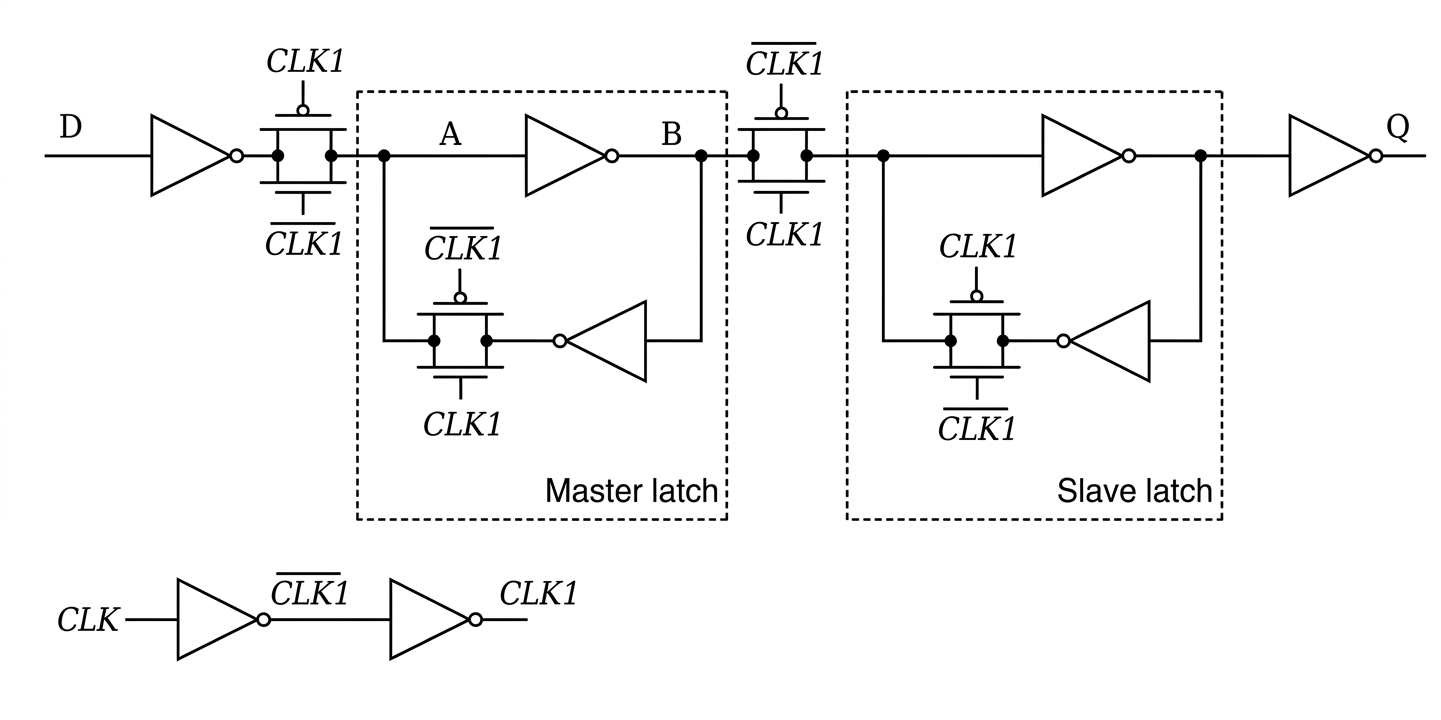
\includegraphics[width=0.60\linewidth]{flipflop_ms.png}
  \caption{主从触发器结构示意。这里不追求内部电路细节，重点是建立“电平敏感”和“边沿敏感”的语义差异。}
\end{figure}

多个寄存器串起来，就形成寄存器链。它可以用于流水线切分路径，也可以用于同步跨域输入。不要把“寄存器链”看成只是几个方框排在一起；每多一级寄存器，系统就多出一个时间边界，也多出一次重新稳定和重新解释数据的机会。

\subsection{寄存器边界与组合逻辑锥}

同步数字系统最常见的结构视角，可以压缩成一句话：寄存器发射数据，组合逻辑做计算，寄存器捕获结果。这就是常说的寄存器到寄存器（register-to-register）路径。中间那片被组合逻辑覆盖的区域，常被描述为一个组合逻辑锥（logic cone），因为从多个输入源看向某个终点寄存器时，逻辑连接常常呈现出逐层汇聚的锥形结构。

\begin{figure}[h]
  \centering
  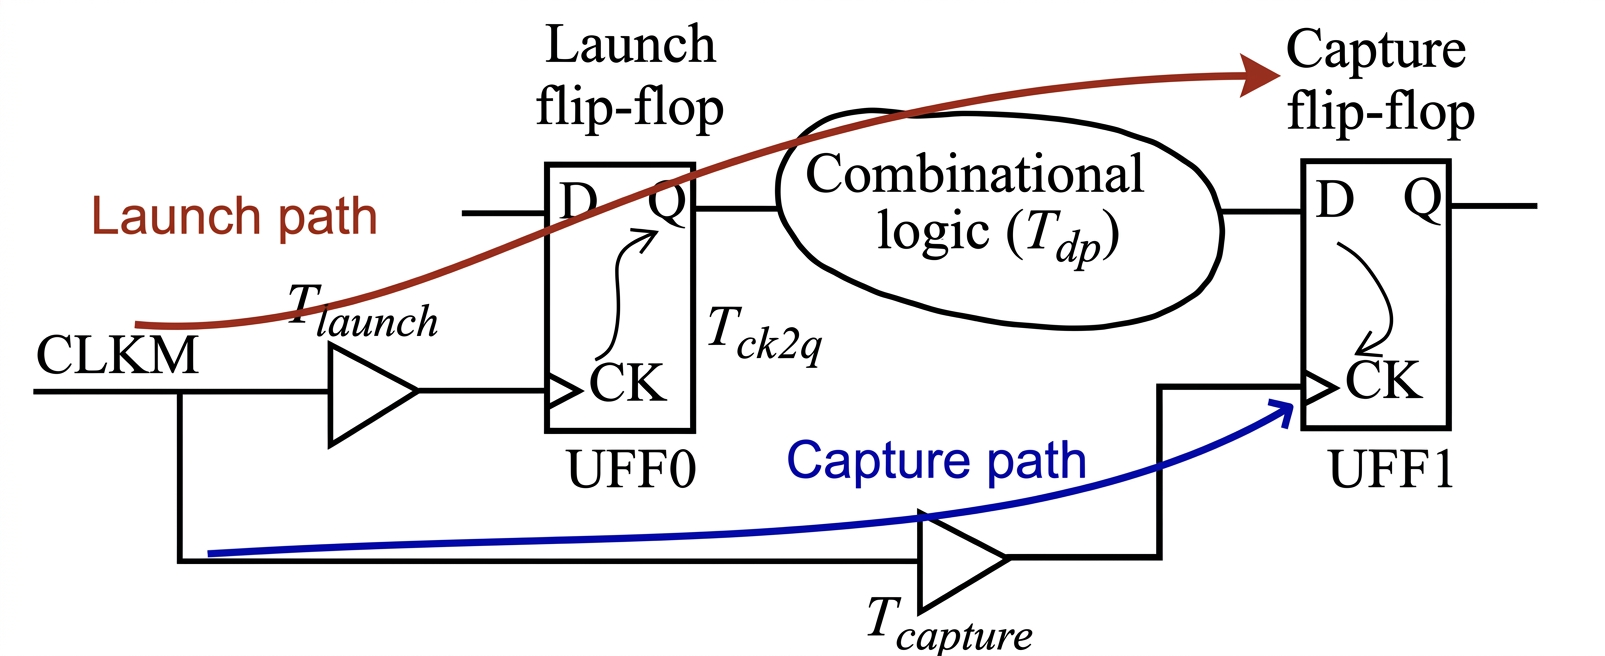
\includegraphics[width=0.64\linewidth]{reg_logic_reg.png}
  \caption{寄存器-组合逻辑-寄存器的基本观察框架。时序约束、路径分析和流水线切分，都建立在这条骨架上。}
\end{figure}

这个视角非常重要，因为它把复杂系统里的很多判断都统一了。路径太长，setup 压力会变大；路径太短，hold 风险可能出现；逻辑锥太深，边沿前收敛可能来不及；跨域输入进入寄存器链，则是在重新定义同步边界。只要把系统先还原成寄存器边界和组合逻辑锥，很多后续术语就不再漂浮。

\subsection{状态机：状态寄存器 + 组合逻辑}

状态机是时序逻辑最标准、也最普遍的组织方式之一。最小骨架只有三部分：状态寄存器保存当前状态；下一状态逻辑根据当前状态和输入计算下一个状态；输出逻辑则根据状态，或者根据状态与输入共同决定对外输出。Moore 机与 Mealy 机的区别就落在这里：前者的输出更直接地挂在状态上，后者的输出还会更紧地受输入影响。

\begin{figure}[h]
  \centering
  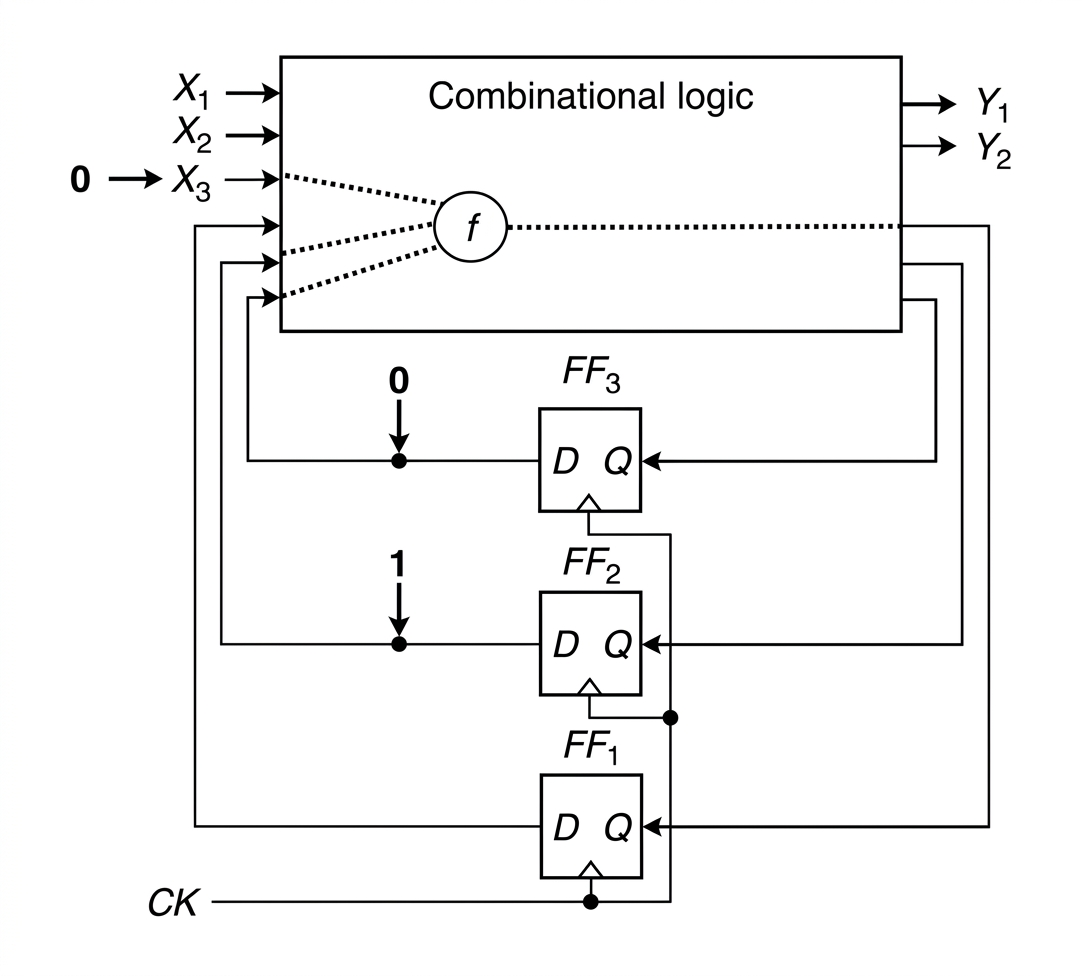
\includegraphics[width=0.62\linewidth]{mealy.jpeg}
  \caption{状态机结构示意。Moore / Mealy 的区别，不只是定义不同，而是输出变化路径与风险暴露点不同。}
\end{figure}

这里不需要急着做复杂状态编码优化。第一遍更重要的是学会识别：什么属于状态、什么属于组合逻辑、什么只是输入条件。很多设计一旦写到 RTL 里变乱，往往不是语法先出问题，而是这三者在脑中没有先分开。

\subsection{Setup / Hold：同步系统的时间边界}

建立时间（setup time）与保持时间（hold time）定义了触发器希望在采样边沿附近看到怎样的数据行为。前者要求数据在采样前提前稳定一段时间，后者要求数据在采样后继续保持一段时间。这不是厂商手册里“形式上列出来的参数”，而是触发器内部电路要可靠完成判决所需要的物理窗口。

\begin{figure}[h]
  \centering
  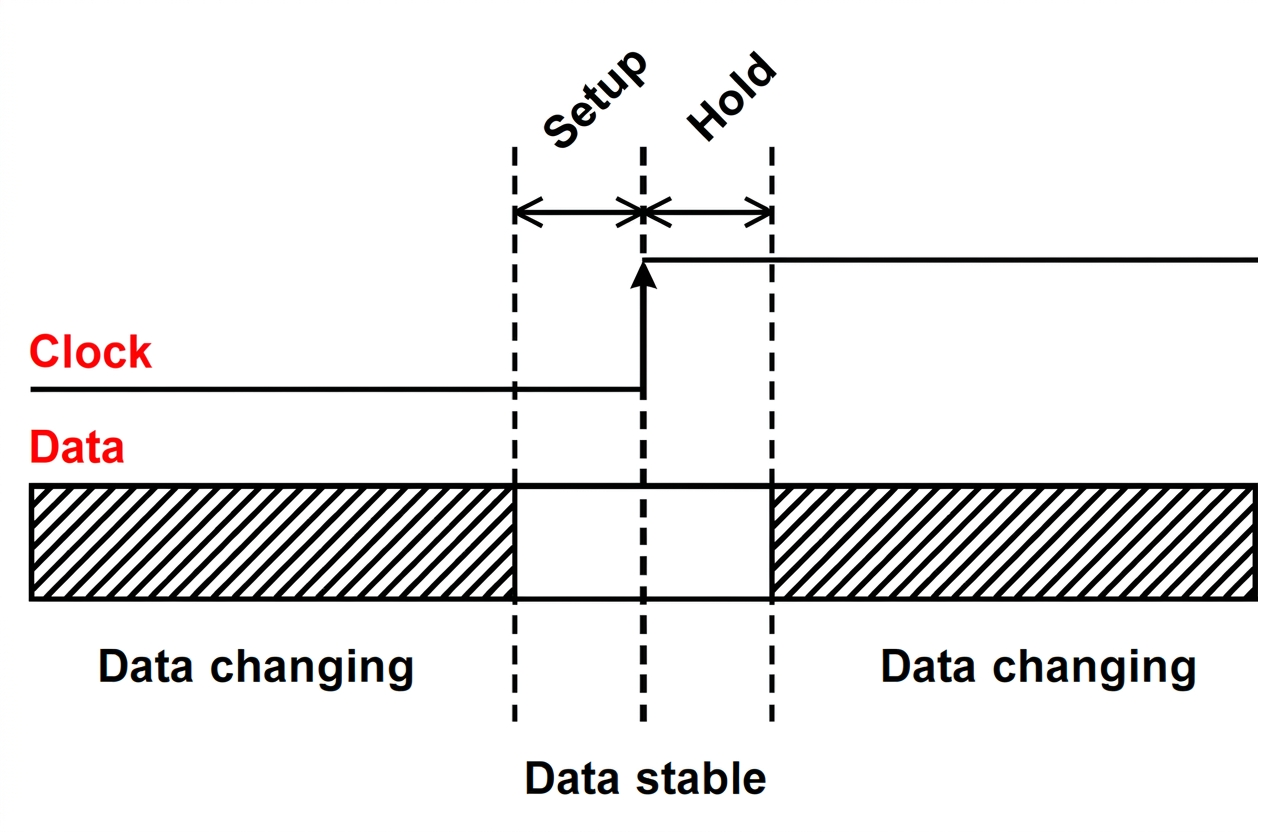
\includegraphics[width=0.68\linewidth]{setup_hold.png}
  \caption{Setup / hold 窗口示意。触发器不是无限快、无限理想的采样器，它需要一个受保护的采样窗口。}
\end{figure}

当数据路径太慢、时钟周期太短、时钟到达差异太不利时，setup 违例就会出现：边沿来了，但正确数据还没到。反过来，当数据路径太快，或者终点寄存器看到时钟太晚时，hold 违例就可能出现：边沿刚过，新数据就抢着冲进来，污染了本应保持的旧数据。两类问题都和“时间窗口被破坏”有关，但破坏方式并不相同，因此修复方法也往往不同。

\subsection{Clock Skew 与 Clock Uncertainty}

初学时很容易把时钟想成一条同时覆盖全芯片的理想节拍线，仿佛每个寄存器都在同一瞬间听到同一拍子。现实并非如此。时钟本身也是一张物理网络，它要经过布线、缓冲、扇出和环境扰动才到达每个寄存器。于是，同一时钟边沿到达不同寄存器的时刻会有差异，这就是时钟偏斜（clock skew）。再考虑抖动、建模误差和环境变化，就得到时钟不确定性（uncertainty）。

这一点之所以重要，是因为很多 setup / hold 裕量其实不是纯粹由数据路径决定的，而是由“数据什么时候到”和“时钟什么时候被各个寄存器看到”共同决定的。换句话说，时钟本身也在参与时序问题，而不是站在系统外部发号施令。

\subsection{亚稳态与同步边界}

如果一个异步输入恰好在采样窗口附近变化，触发器内部可能一时无法决定该收敛到 0 还是 1，于是短时间停在一种不稳定的中间状态，这就是亚稳态。它不是第三种稳定逻辑电平，而是一种不稳定、可恢复、但恢复时间不可被完全保证上界的状态。

\begin{figure}[h]
  \centering
  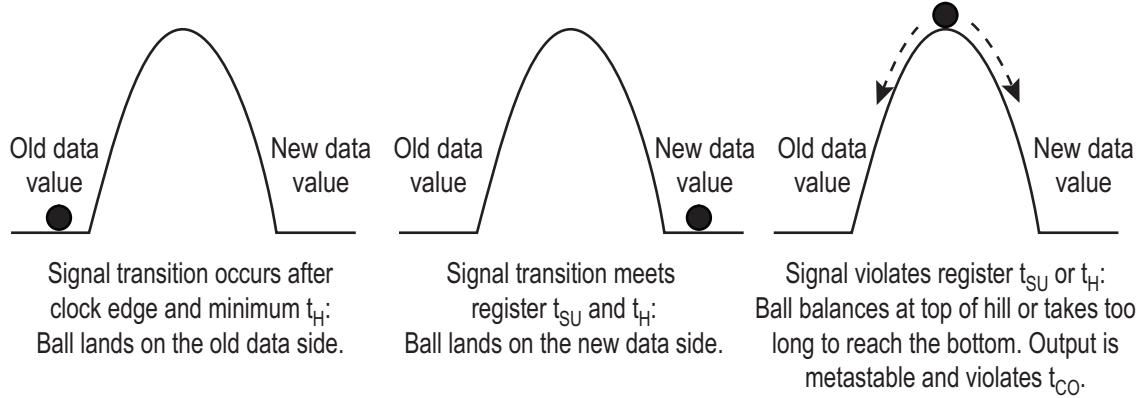
\includegraphics[width=0.58\linewidth]{metastability_description.jpg}
  \caption{亚稳态示意。关键不在于把它神秘化，而在于承认它是采样连续世界时不可彻底消除的概率事件。}
\end{figure}

工程上真正重要的结论是：亚稳态不能被彻底消灭，只能被降低概率。双触发器同步器的核心作用，就是给第一级可能进入亚稳态的触发器多一拍恢复时间，让第二级在更高概率上看到已经稳定的 0 或 1。但它只适用于单 bit 控制信号的最小同步场景；多 bit 总线、握手协议、异步 FIFO 之类的问题，还需要更完整的 CDC 设计策略。

\begin{figure}[h]
  \centering
  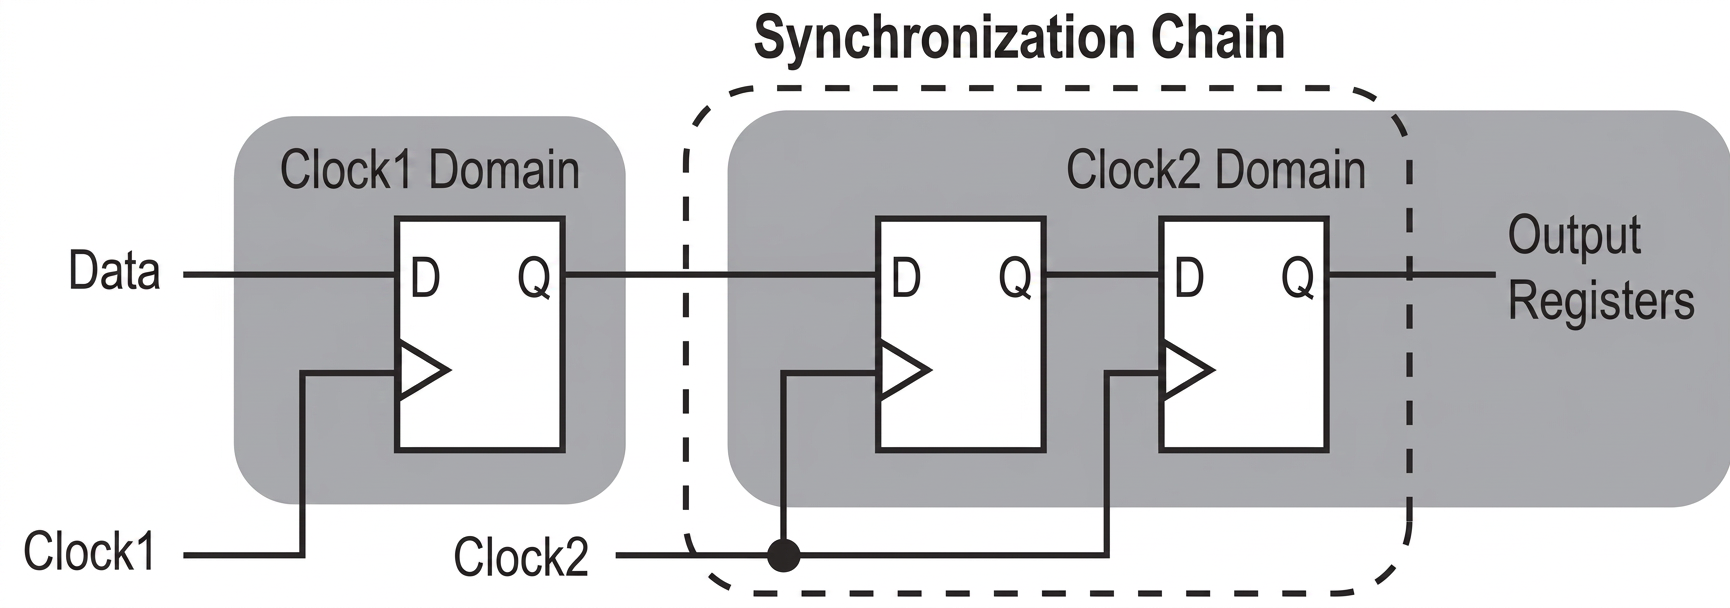
\includegraphics[width=0.55\linewidth]{dual_dff_capture.png}
  \caption{双触发器同步器。它在解决概率问题，而不是自动解决所有跨域协议问题。}
\end{figure}

\section{关键图示或案例}

本讲最值得反复看的图，不是某一页状态图本身，而是那张“寄存器-组合逻辑-寄存器”的骨架图。因为从那张图开始，setup/hold 是在检查什么、状态机的状态存在哪里、跨域风险会从哪里进入、为什么同步器要放在边界上，这些问题都开始有了统一的落脚点。学完之后，如果面对一个新系统，你能先把它抽成几个寄存器边界和几片组合逻辑锥，再去问状态、时序和跨域问题在哪里，那这一讲的核心任务就完成了。

\begin{tipbox}
第一次学时序逻辑时，不必急着把所有术语一次讲透。先抓住三件事：寄存器在制造时间边界，setup / hold 在保护采样窗口，异步输入会挑战这套秩序。后面的 RTL、STA 和 CDC 都会沿着这三条线反复回来加深。
\end{tipbox}

\begin{warnbox}
不要把“同步器”误解成万能胶。双触发器同步器只能降低单 bit 异步输入引发亚稳态传播的概率，不能自动保证多 bit 数据一致性，也不能替代协议设计、握手或异步 FIFO 之类更完整的跨域机制。
\end{warnbox}

\section{本讲小结}

这一讲把系统从“函数”推进成了“状态机”。寄存器引入了历史，也引入了时间边界；setup、hold、skew 与 uncertainty 则定义了这些边界能否被可靠维持；亚稳态和 CDC 则提醒我们，连续世界总会在同步边界上重新闯入数字系统。到这里，第三章真正完成了它的承重任务：既让读者看到逻辑如何从器件世界里长出来，也让读者知道一旦引入寄存器和时钟，系统正确性就必须同时受逻辑关系和时间关系约束。下一章进入 RTL 时，重点就可以自然转向：这些语义边界在 Verilog / SystemVerilog 里应该如何被正确建模。

\section{练习题}

\begin{enumerate}
  \item 画出一个寄存器-组合逻辑-寄存器结构，并在图中标出数据路径、时钟路径、setup 检查窗口和 hold 检查窗口。
  \item 对一个简单自动售货机或交通灯控制器，区分哪些信息属于“状态”，哪些逻辑属于“下一状态逻辑”，哪些属于“输出逻辑”。
  \item 给出一个 setup violation 和一个 hold violation 的场景，分别解释它们更像是哪一类时间窗口被破坏。
  \item 说明为什么异步按键直接进入主时钟域寄存器会有风险；进一步解释双触发器同步器在这里能做什么、不能做什么。
\end{enumerate}

\end{document}
